
%(BEGIN_QUESTION)
% Copyright 2011, Tony R. Kuphaldt, released under the Creative Commons Attribution License (v 1.0)
% This means you may do almost anything with this work of mine, so long as you give me proper credit

Examine these two pneumatic control ``loops'' (transmitter-controller-valve systems) for an industrial boiler, controlling both water level and steam pressure:

$$\includegraphics[width=15.5cm]{i00478x01.eps}$$

If the PIC setpoint is 225 PSI and the measured pressure begins to fall below that value, how should the PIC respond, and how will this response bring the steam pressure back up to setpoint?

\vskip 10pt

If the pump supplying feedwater to the boiler begins to wear down over time, becoming less and less effective at providing water pressure to the level control valve, how do you suspect the LIC will respond over time as it works to maintain steam drum water level at setpoint?

\vskip 10pt

Describe a situation where {\it manual mode} might be useful to either the boiler operator, or to an instrument technician tasked with maintaining either of these control loops.

\vskip 10pt

Suppose the level transmitter's calibration was 12 to 22 inches of water level while the level indicating controller's calibration was 10 to 20 inches of water level.  How many inches of water level would the LIC indicate when the actual steam drum water level was 17 inches?  

\underbar{file i00478}
%(END_QUESTION)





%(BEGIN_ANSWER)

If pressure falls, PIC should increase fuel to burner.

\vskip 10pt

As feedwater pump wears, LIC should open valve more.

\vskip 10pt

The operator could use manual mode to gradually heat boiler during start-up, or to shut it down.

\vskip 10pt

I'll let you figure out what the LIC would indicate!

%(END_ANSWER)





%(BEGIN_NOTES)

If steam pressure begins to fall below setpoint, the PIC should send an increasing signal to the fuel gas valve, causing the burner to output more heat and thereby raising the steam pressure to setpoint again.  If well-tuned, a loop controller will drive its output signal to {\it whatever value is necessary} to achieve PV = SP.

\vskip 10pt

As the feedwater pump wears, the level control valve will have to open up over time to achieve the same water flow rate into the boiler, all other factors being equal.  Thus, the LIC outputs a signal that is slightly greater as time goes on, in order to compensate for the mechanical changes happening in the feedwater pump.

\vskip 10pt

Manual mode would be useful for the following scenarios:

\begin{itemize}
\item{} Briefly ``stroke-testing'' either control valve to check for proper stem motion
\item{} Holding either control valve in a set position while the transmitter was disconnected from the controller for maintenance purposes
\item{} Introducing a ``step-change'' disturbance into the boiler by placing the controller in manual and then ``bumping'' the output signal either up or down just a bit, observing the process variable response over time to learn how the boiler naturally responds to such a change.
\end{itemize}

\vskip 10pt

When the actual water level was 17 inches (signal pressure = 9 PSI = 50\%), the LIC would register 15 inches (50\% of range).









\vskip 20pt \vbox{\hrule \hbox{\strut \vrule{} {\bf Suggestions for Socratic discussion} \vrule} \hrule}

\begin{itemize}
\item{} If the LT outputs a 9 PSI (50\%) signal, what position will the feedwater control valve be in?  If we cannot tell, identify the missing information.
\item{} What would happen in this system if the PT failed with a high signal, with the PIC in automatic mode?
\item{} What would happen in this system if the fuel gas supply line got shut off, with the PIC in automatic mode?
\item{} What would happen in this system if the feedwater pump suddenly stopped, with the LIC in automatic mode?
\item{} What would happen in this system if the feedwater pump suddenly stopped, with the LIC in manual mode?
\end{itemize}










\filbreak \vskip 20pt \vbox{\hrule \hbox{\strut \vrule{} {\bf Virtual Troubleshooting} \vrule} \hrule}

\noindent
{\bf Predicting the effect of a given fault:} present each of the following faults to the students, one at a time, having them comment on all the effects each fault would produce.

\begin{itemize}
\item{} Air supply pressure to LIC fails (0 PSI) 
\item{} Air supply pressure to PIC fails (0 PSI) 
\item{} Air tube between LT and LIC leaks (fails vented)
\item{} Air tube between PT and PIC leaks (fails vented)
\item{} Fuel gas supply pressure falls well below normal
\end{itemize}


\vskip 10pt


\noindent
{\bf Determining the utility of given diagnostic tests:} imagine the pressure transmitter fails with a high signal ($>$ 15 PSI output) in this system (but don't tell this to students!).  Present the operator's observation(s) to the students, have them consider possible faults and diagnostic strategies, and then propose the following diagnostic tests one by one.  Have students rate the value of each test, determining whether or not each test would give us useful information (i.e. tell us something we don't already know).  Also have students describe what re

\begin{itemize}
\item{} {\it PT failed high, PIC sends 0\% signal to fuel gas valve}
\item{} Place PIC in manual mode and raise output signal while watching PV display -- {\bf No}
\item{} Place PIC in manual mode and change output signal while watching control valve -- {\bf Yes}
\item{} Check reading of flow transmitter somewhere upstream in the fuel gas line -- {\bf Yes}
\item{} Place LIC in manual mode and change output signal while watching PIC reading -- {\bf No}
\end{itemize}


\vskip 10pt


\noindent
{\bf Diagnosing a fault based on given symptoms:} imagine the air supply to the LIC fails (0 PSI) in this system (but don't tell this to students!).  Present the operator's observation(s) to the students, have them consider possible faults and diagnostic strategies, and then tell them the results of tests they propose based on the following symptoms, until they have properly identified the nature and location of the fault:

\begin{itemize}
\item{} {\it Operator sees the LIC's PV begin to fall below SP, as the control valve shuts off and the boiler runs out of water}
\end{itemize}

%INDEX% Basics, control loop troubleshooting: determining effect of specified fault(s)

%(END_NOTES)


